%!TEX root = forallxsol.tex
%\part{Natural deduction for FOL}
%\label{ch.NDFOL}
%\addtocontents{toc}{\protect\mbox{}\protect\hrulefill\par}

\setcounter{chapter}{31}
\chapter{Basic rules for FOL}\setcounter{ProbPart}{0}
\problempart
Explain why these two `proofs' are incorrect. Also, provide interpretations which would invalidate the fallacious argument forms the `proofs' enshrine:
\begin{multicols}{2}
	\begin{fitchproof}
		\hypo{Rxx}{\forall x\,\atom{R}{x,x}}
		\have{Raa}{\atom{R}{a,a}}\Ae{Rxx}
		\have{Ray}{\forall y\,\atom{R}{a,y}}\Ai{Raa}
		\have{Rxy}{\forall x \forall y\,\atom{R}{x,y}}\Ai{Ray}
	\end{fitchproof}
\vfill
\noindent\myanswer{When using $\forall$I, you must replace \emph{all} names with the new variable. So line 3 is bogus. As a counterinterpretation, consider the following:
\begin{center}
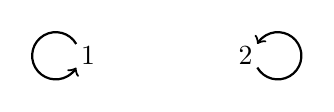
\begin{tikzpicture}
\node (atom4) at (0,0) {1};
\node (atom5) at (2,0) {2};
\draw[->, thick] (atom4)+(-0.15,0.15) arc (-330:-30:.3); 
\draw[->, thick] (atom5)+(0.15,-0.15) arc (-150:150:.3); 
\end{tikzpicture}
\end{center}}
\columnbreak
	\begin{fitchproof}
		\hypo{AE}{\forall x \exists y\,\atom{R}{x,y}}
		\have{E}{\exists y\,\atom{R}{a,y}}\Ae{AE}
		\open
			\hypo{ass}{\atom{R}{a,a}}
			\have{Ex}{\exists x\,\atom{R}{x,x}}\Ei{ass}
		\close
		\have{con}{\exists x\,\atom{R}{x,x}}\Ee{E, ass-Ex}
	\end{fitchproof}
\vfill
\noindent\myanswer{The instantiating constant, `$a$', occurs in the line (line 2) to which $\exists$E is to be applied on line 5. So the use of $\exists$E on line 5 is bogus. As a counterinterpretation, consider the following:
\begin{center}
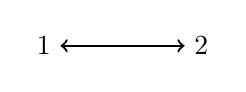
\begin{tikzpicture}
\node (atom4) at (0,0) {1};
\node (atom5) at (2,0) {2};
\draw[<->, thick] (atom4)--(atom5);
\end{tikzpicture}
\end{center}}
\end{multicols}


\problempart 
\label{pr.justifyFOLproof}
The following three proofs are missing their citations (rule and line numbers). Add them, to turn them into bona fide proofs. 
\begin{earg}
\item\begin{fitchproof}
\hypo{p1}{\forall x\exists y(\atom{R}{x,y} \eor \atom{R}{y,x})}
\hypo{p2}{\forall x\enot \atom{R}{m,x}}
\have{3}{\exists y(\atom{R}{m,y} \eor \atom{R}{y,m})}\Ae{p1}
	\open
		\hypo{a1}{\atom{R}{m,a} \eor \atom{R}{a,m}}
		\have{a2}{\enot \atom{R}{m,a}}\Ae{p2}
		\have{a3}{\atom{R}{a,m}}\ds{a1, a2}
		\have{a4}{\exists x\,\atom{R}{x,m}}\Ei{a3}
	\close
\have{n}{\exists x\,\atom{R}{x,m}}\Ee{3, a1-a4}
\end{fitchproof}

\item\begin{fitchproof}
\hypo{1}{\forall x(\exists y\,\atom{L}{x,y} \eif \forall z\atom{L}{z,x})}
\hypo{2}{\atom{L}{a,b}}
\have{3}{\exists y\,\atom{L}{a,y} \eif \forall z\atom{L}{z,a}}\Ae{1}
\have{4}{\exists y\,\atom{L}{a,y}}\Ei{2}
\have{5}{\forall z \atom{L}{z,a}}\ce{3, 4}
\have{6}{\atom{L}{c,a}}\Ae{5}
\have{7}{\exists y\,\atom{L}{c,y} \eif \forall z\atom{L}{z,c}}\Ae{1}
\have{8}{\exists y\,\atom{L}{c,y}}\Ei{6}
\have{9}{\forall z \atom{L}{z,c}}\ce{7, 8}
\have{10}{\atom{L}{c,c}}\Ae{9}
\have{11}{\forall x\,\atom{L}{x,x}}\Ai{10}
\end{fitchproof}

\item\begin{fitchproof}
\hypo{a}{\forall x(\atom{J}{x} \eif \atom{K}{x})}
\hypo{b}{\exists x\forall y\,\atom{L}{x,y}}
\hypo{c}{\forall x\,\atom{J}{x}}
\open
	\hypo{2}{\forall y\,\atom{L}{a,y}}
	\have{3}{\atom{L}{a,a}}\Ae{2}
	\have{d}{\atom{J}{a}}\Ae{c}
	\have{e}{\atom{J}{a} \eif \atom{K}{a}}\Ae{a}
	\have{f}{\atom{K}{a}}\ce{e, d}
	\have{4}{\atom{K}{a} \eand \atom{L}{a,a}}\ai{f, 3}
	\have{5}{\exists x(\atom{K}{x} \eand \atom{L}{x,x})}\Ei{4}
\close
\have{j}{\exists x(\atom{K}{x} \eand \atom{L}{x,x})}\Ee{b, 2-5}
\end{fitchproof}
\end{earg}


\problempart
\label{pr.BarbaraEtc.proof1}
In \S\ref{s:MoreMonadic} problem A, we considered fifteen syllogistic figures of Aristotelian logic. Provide proofs for each of the argument forms. NB: You will find it \emph{much} easier if you symbolize (for example) `No F is G' as `$\forall x (\atom{F}{x} \eif \enot \atom{G}{x})$'.
\\\myanswer{We prove the four Figure I syllogisms; the rest are \emph{extremely} similar.
\begin{multicols}{2}
\noindent \textbf{Barbara}
\begin{fitchproof}
\hypo{gf}{\forall x (\atom{G}{x} \eif \atom{F}{x})}
\hypo{hg}{\forall x (\atom{H}{x} \eif \atom{G}{x})}
\have{gafa}{\atom{G}{a} \eif \atom{F}{a}}\Ae{gf}
\have{haga}{\atom{H}{a} \eif \atom{G}{a}}\Ae{hg}
\open
	\hypo{ha}{\atom{H}{a}}
	\have{ga}{\atom{G}{a}}\ce{haga, ha}
	\have{fa}{\atom{F}{a}}\ce{gafa, ga}
\close
\have{hafa}{\atom{H}{a} \eif \atom{F}{a}}\ci{ha-fa}
\have{con}{\forall x (\atom{H}{x} \eif \atom{F}{x})}\Ai{hafa}
\end{fitchproof}
\vfill
\noindent\textbf{Celerant} is exactly as Barbara, replacing `$F$' with `$\enot F$' throughout.
\columnbreak
\\\textbf{Ferio} 
\begin{fitchproof}
\hypo{gnf}{\forall x (\atom{G}{x} \eif \enot \atom{F}{x})}
\hypo{hg}{\exists x (\atom{H}{x} \eand  \atom{G}{x})}
\open
	\hypo{haga}{\atom{H}{a} \eand \atom{G}{a}}
	\have{ha}{\atom{H}{a}}\ae{haga}
	\have{ga}{\atom{G}{a}}\ae{haga}
	\have{ganfa}{\atom{G}{a} \eif \enot \atom{F}{a}}\Ae{gnf}
	\have{nfa}{\enot \atom{F}{a}}\ce{ganfa, ga}
	\have{hanfa}{\atom{H}{a} \eand \enot \atom{F}{a}}\ai{ha, nfa}
	\have{hnf}{\exists x (\atom{H}{x} \eand \enot \atom{F}{x})}\Ei{hanfa}
\close
\have{con}{\exists x (\atom{H}{x} \eand \enot \atom{F}{x})}\Ee{hg, haga-hnf}
\end{fitchproof}
\\\textbf{Darii} is exactly as Ferio, replacing `$\enot F$' with `$F$' throughout.\end{multicols}}

\

\problempart
\label{pr.BarbaraEtc.proof2}
Aristotle and his successors identified other syllogistic forms which depended upon `existential import'. Symbolize each of the following argument forms in FOL and offer proofs.
\begin{earg}
\newpage	\item \textbf{Barbari.} Something is H. All G are F. All H are G. So: Some H is F
	\\\myanswer{$\exists x\,\atom{H}{x}, \forall x(\atom{G}{x} \eif \atom{F}{x}), \forall x (\atom{H}{x} \eif \atom{G}{x}) \therefore \exists x (\atom{H}{x} \eand \atom{F}{x})$
\begin{fitchproof}
\hypo{imp}{\exists x\,\atom{H}{x}}
\hypo{gf}{\forall x (\atom{G}{x} \eif \atom{F}{x})}
\hypo{hg}{\forall x (\atom{H}{x} \eif \atom{G}{x})}
\open
	\hypo{ha}{\atom{H}{a}}
	\have{haga}{\atom{H}{a} \eif \atom{G}{a}}\Ae{hg}
	\have{ga}{\atom{G}{a}}\ce{haga, ha}
	\have{gafa}{\atom{G}{a} \eif \atom{F}{a}}\Ae{gf}
	\have{fa}{\atom{F}{a}}\ce{gafa, ga}
	\have{hafa}{\atom{H}{a} \eand \atom{F}{a}}\ai{ha, fa}
	\have{hf}{\exists x (\atom{H}{x} \eand \atom{F}{x})}\Ei{hafa}
\close
\have{con}{\exists x (\atom{H}{x} \eand \atom{F}{x})}\Ee{imp, ha-hf}
\end{fitchproof}}
	
	\item \textbf{Celaront.} Something is H. No G are F. All H are G. So: Some H is not F
	\\\myanswer{$\exists x\,\atom{H}{x}, \forall x(\atom{G}{x} \eif \enot \atom{F}{x}), \forall x (\atom{H}{x} \eif \atom{G}{x}) \therefore \exists x (\atom{H}{x} \eand \enot \atom{F}{x})$
\\	Proof is exactly as for Barbari, replacing `$F$' with `$\enot F$' throughout.}
	\item \textbf{Cesaro.} Something is H. No F are G. All H are G. So: Some H is not F.
	\\\myanswer{$\exists x\,\atom{H}{x}, \forall x(\atom{F}{x} \eif \enot \atom{G}{x}), \forall x (\atom{H}{x} \eif \atom{G}{x}) \therefore \exists x (\atom{H}{x} \eand \enot \atom{F}{x})$
\begin{fitchproof}
\hypo{imp}{\exists x\,\atom{H}{x}}
\hypo{fg}{\forall x (\atom{F}{x} \eif \enot \atom{G}{x})}
\hypo{hng}{\forall x (\atom{H}{x} \eif  \atom{G}{x})}
\open
	\hypo{ha}{\atom{H}{a}}
	\have{hanga}{\atom{H}{a} \eif \atom{G}{a}}\Ae{hng}
	\have{nga}{\atom{G}{a}}\ce{hanga, ha}
	\have{faga}{\atom{F}{a} \eif \enot \atom{G}{a}}\Ae{fg}
	\open
		\hypo{fa}{\atom{F}{a}}
		\have{ga}{\enot \atom{G}{a}}\ce{faga, fa}
		\have{red}{\ered}\ri{nga, ga}
	\close
	\have{nfa}{\enot \atom{F}{a}}\ni{fa-red}
	\have{hanfa}{\atom{H}{a} \eand \enot \atom{F}{a}}\ai{ha, nfa}
	\have{hnf}{\exists x (\atom{H}{x} \eand \enot \atom{F}{x})}\Ei{hanfa}
\close
\have{con}{\exists x (\atom{H}{x} \eand \enot \atom{F}{x})}\Ee{imp, ha-hnf}
\end{fitchproof}
}
\newpage	\item \textbf{Camestros.} Something is H. All F are G. No H are G. So: Some H is not F.
	\\\myanswer{$\exists x\,\atom{H}{x}, \forall x(\atom{F}{x} \eif \atom{G}{x}), \forall x (\atom{H}{x} \eif \enot \atom{G}{x}) \therefore \exists x (\atom{H}{x} \eand \enot \atom{F}{x})$
\begin{fitchproof}
\hypo{imp}{\exists x\,\atom{H}{x}}
\hypo{fg}{\forall x (\atom{F}{x} \eif \atom{G}{x})}
\hypo{hng}{\forall x (\atom{H}{x} \eif \enot \atom{G}{x})}
\open
	\hypo{ha}{\atom{H}{a}}
	\have{hanga}{\atom{H}{a} \eif \enot \atom{G}{a}}\Ae{hng}
	\have{nga}{\enot \atom{G}{a}}\ce{hanga, ha}
	\have{faga}{\atom{F}{a} \eif \atom{G}{a}}\Ae{fg}
	\have{nfa}{\enot \atom{F}{a}}\mt{faga, nga}
	\have{hanfa}{\atom{H}{a} \eand \enot \atom{F}{a}}\ai{ha, nfa}
	\have{hnf}{\exists x (\atom{H}{x} \eand \enot \atom{F}{x})}\Ei{hanfa}
\close
\have{con}{\exists x (\atom{H}{x} \eand \enot \atom{F}{x})}\Ee{imp, ha-hnf}
\end{fitchproof}}

	\item \textbf{Felapton.} Something is G. No G are F. All G are H. So: Some H is not F.
	\\\myanswer{$\exists x\,\atom{G}{x}, \forall x (\atom{G}{x} \eif \enot \atom{F}{x}), \forall x(\atom{G}{x} \eif \atom{H}{x}) \therefore \exists x (\atom{H}{x} \eand \enot \atom{F}{x})$
\begin{fitchproof}
\hypo{imp}{\exists x\,\atom{G}{x}}
\hypo{gnf}{\forall x (\atom{G}{x} \eif \enot \atom{F}{x})}
\hypo{gh}{\forall x (\atom{G}{x} \eif \atom{H}{x})}
\open
	\hypo{ga}{\atom{G}{a}}
	\have{gaha}{\atom{G}{a} \eif \atom{H}{a}}\Ae{gh}
	\have{ha}{\atom{H}{a}}\ce{gaha, ga}
	\have{ganfa}{\atom{G}{a} \eif \enot \atom{F}{a}}\Ae{gnf}
	\have{nfa}{\enot \atom{F}{a}}\ce{ganfa, ga}
	\have{hanfa}{\atom{H}{a} \eand \enot \atom{F}{a}}\ai{ha, nfa}
	\have{hnf}{\exists x (\atom{H}{x} \eand \enot \atom{F}{x})}\Ei{hanfa}
\close
\have{con}{\exists x (\atom{H}{x} \eand \atom{F}{x})}\Ee{imp, ga-hnf}
\end{fitchproof}}
	\item \textbf{Darapti.} Something is G. All G are F. All G are H. So: Some H is F.
	\\\myanswer{$\exists x\,\atom{G}{x}, \forall x (\atom{G}{x} \eif \atom{F}{x}), \forall x(\atom{G}{x} \eif \atom{H}{x}) \therefore \exists x (\atom{H}{x} \eand \atom{F}{x})$\\
	Proof is exactly as for Felapton, replacing `$\enot F$' with `$F$' throughout.}

\newpage	\item \textbf{Calemos.} Something is H. All F are G. No G are H. So: Some H is not F.
	\\\myanswer{$\exists x\,\atom{H}{x}, \forall x(\atom{F}{x} \eif \atom{G}{x}), \forall x(\atom{G}{x} \eif \enot \atom{H}{x}) \therefore \exists x (\atom{H}{x} \eand \enot \atom{F}{x})$
\begin{fitchproof}
\hypo{imp}{\exists x\,\atom{H}{x}}
\hypo{fg}{\forall x (\atom{F}{x} \eif \atom{G}{x})}
\hypo{gnh}{\forall x (\atom{G}{x} \eif \enot \atom{H}{x})}
\open
	\hypo{ha}{\atom{H}{a}}
	\have{ganha}{\atom{G}{a} \eif \enot \atom{H}{a}}\Ae{gnh}
	\open
		\hypo{ga}{\atom{G}{a}}
		\have{nha}{\enot \atom{H}{a}}\ce{ganha, ga}
		\have{red}{\ered}\ri{ha, nha}
	\close
	\have{nga}{\enot \atom{G}{a}}\ni{ga-red}
	\have{faga}{\atom{F}{a} \eif \atom{G}{a}}\Ae{fg}
	\have{nfa}{\enot \atom{F}{a}}\mt{faga, nga}
	\have{hanfa}{\atom{H}{a} \eand \enot \atom{F}{a}}\ai{ha, nfa}
	\have{hnf}{\exists x (\atom{H}{x} \eand \atom{F}{x})}\Ei{hanfa}
\close
\have{con}{\exists x (\atom{H}{x} \eand \atom{F}{x})}\Ee{imp, ha-hnf}
\end{fitchproof}}
	
	\item \textbf{Fesapo.} Something is G. No F is G. All G are H. So: Some H is not F.
	\\\myanswer{$\exists x\,\atom{G}{x}, \forall x(\atom{F}{x} \eif \enot \atom{G}{x}), \forall x(\atom{G}{x} \eif \atom{H}{x}) \therefore \exists x (\atom{H}{x} \eand \enot \atom{F}{x})$
	\begin{fitchproof}
\hypo{imp}{\exists x\,\atom{G}{x}}
\hypo{fng}{\forall x (\atom{F}{x} \eif \enot \atom{G}{x})}
\hypo{gh}{\forall x (\atom{G}{x} \eif \atom{H}{x})}
\open
	\hypo{ga}{\atom{G}{a}}
	\have{gaha}{\atom{G}{a} \eif  \atom{H}{a}}\Ae{gh}
	\have{ha}{\atom{H}{a}}\ce{gaha, ga}
	\have{fanga}{\atom{F}{a} \eif \enot \atom{G}{a}}\Ae{fng}
	\open
		\hypo{fa}{\atom{F}{a}}
		\have{nga}{\enot \atom{G}{a}}\ce{fanga, fa}
		\have{red}{\ered}\ri{ga, nga}
	\close
	\have{nfa}{\enot \atom{F}{a}}\ni{fa-red}
	\have{hanfa}{\atom{H}{a} \eand \enot \atom{F}{a}}\ai{ha, nfa}
	\have{hnf}{\exists x (\atom{H}{x} \eand \enot \atom{F}{x})}\Ei{hanfa}
\close
\have{con}{\exists x (\atom{H}{x} \eand \enot \atom{F}{x})}\Ee{imp, ga-hnf}
\end{fitchproof}}

\newpage	\item \textbf{Bamalip.} Something is F. All F are G. All G are H. So: Some H are F.
	\\\myanswer{$\exists x\,\atom{F}{x}, \forall x(\atom{F}{x} \eif \atom{G}{x}), \forall x(\atom{G}{x} \eif \atom{H}{x}) \therefore \exists x (\atom{H}{x} \eand \atom{F}{x})$
\begin{fitchproof}
\hypo{imp}{\exists x\,\atom{F}{x}}
\hypo{fg}{\forall x (\atom{F}{x} \eif \atom{G}{x})}
\hypo{gh}{\forall x (\atom{G}{x} \eif \atom{H}{x})}
\open
	\hypo{fa}{\atom{F}{a}}
	\have{faga}{\atom{F}{a} \eif \atom{G}{a}}\Ae{fg}
	\have{ga}{\atom{G}{a}}\ce{faga, fa}
	\have{gaha}{\atom{G}{a} \eif \atom{H}{a}}\Ae{gh}
	\have{ha}{\atom{H}{a}}\ce{gaha, ga}
	\have{hafa}{\atom{H}{a} \eand \atom{F}{a}}\ai{ha, fa}
	\have{hf}{\exists x (\atom{H}{x} \eand \atom{F}{x})}\Ei{hafa}
\close
\have{con}{\exists x (\atom{H}{x} \eand \atom{F}{x})}\Ee{imp, fa-hf}
\end{fitchproof}}
\end{earg}

\problempart
\label{pr.someFOLproofs}
Provide a proof of each claim.
\begin{earg}
\item $\proves \forall x\,\atom{F}{x} \eif \forall y(\atom{F}{y} \eand \atom{F}{y})$
\myanswer{\begin{fitchproof}
\open
	\hypo{Af}{\forall x\,\atom{F}{x}}
	\have{con}{\atom{F}{a}}\Ae{Af}
	\have{con2}{\atom{F}{a} \eand \atom{F}{a}}\ai{con,con}
	\have{con3}{\forall y\,(\atom{F}{y} \eand \atom{F}{y})}\Ai{con2}
\close
\have{con4}{\forall x\,\atom{F}{x} \eif \forall y(\atom{F}{x} \eand \atom{F}{x})}\ci{Af-con3}
\end{fitchproof}}

\item $\forall x(Ax\eif \atom{B}{x}), \exists x\,\atom{A}{x} \proves \exists x\,\atom{B}{x}$
\myanswer{\begin{fitchproof}
\hypo{Aab}{\forall x (\atom{A}{x} \eif \atom{B}{x})}
\hypo{Ea}{\exists x\,\atom{A}{x}}
\open
	\hypo{a}{\atom{A}{a}}
	\have{ab}{\atom{A}{a} \eif \atom{B}{a}}\Ae{Aab}
	\have{b}{\atom{B}{a}}\ce{ab, a}
	\have{Eb}{\exists x\,\atom{B}{x}}\Ei{b}
\close
\have{Eb1}{\exists x\,\atom{B}{x}}\Ee{Ea, a-Eb}
\end{fitchproof}}

\newpage\item $\forall x(\atom{M}{x} \eiff \atom{N}{x}), \atom{M}{a} \eand \exists x\,\atom{R}{x,a}\proves \exists x\,\atom{N}{x}$
\myanswer{\begin{fitchproof}
\hypo{Amn}{\forall x (\atom{M}{x} \eiff \atom{N}{x})}
\hypo{mEr}{\atom{M}{a} \eand \exists x\,\atom{R}{x,a}}
\have{m}{\atom{M}{a}}\ae{mEr}
\have{mn}{\atom{M}{a} \eiff \atom{N}{a}}\Ae{Amn}
\have{n}{\atom{N}{a}}\be{mn, m}
\have{En}{\exists x\,\atom{N}{x}}\Ei{n}
\end{fitchproof}}

\item $\forall x \forall y\,\atom{G}{x,y}\proves\exists x\,\atom{G}{x,x}$
\myanswer{\begin{fitchproof}
\hypo{AAg}{\forall x \forall y\,\atom{G}{x,y}}
\have{Ag}{\forall y\,\atom{G}{a,y}}\Ae{AAg}
\have{g}{\atom{G}{a,a}}\Ae{Ag}
\have{Eg}{\exists x\,\atom{G}{x,x}}\Ei{g}
\end{fitchproof}}

\item $\proves\forall x\,\atom{R}{x,x}\eif \exists x \exists y\,\atom{R}{x,y}$
\myanswer{\begin{fitchproof}
\open
	\hypo{Ar}{\forall x\,\atom{R}{x,x}}
	\have{r}{\atom{R}{a,a}}\Ae{Ar}
	\have{Er}{\exists y\,\atom{R}{a,y}}\Ei{r}
	\have{EEr}{\exists x \exists y\,\atom{R}{x,y}}\Ei{Er}
\close
\have{ArEEr}{\forall x\,\atom{R}{x,x} \eif \exists x \exists y\,\atom{R}{x,y}}\ci{Ar-EEr}
\end{fitchproof}}

\item $\proves\forall y \exists x (\atom{Q}{y} \eif \atom{Q}{x})$
\myanswer{\begin{fitchproof}
\open
	\hypo{q}{\atom{Q}{a}}
	\have{q1}{\atom{Q}{a}}\by{R}{q}
\close
\have{qq}{\atom{Q}{a} \eif \atom{Q}{a}}\ci{q-q1}
\have{Eqq}{\exists x(\atom{Q}{a} \eif \atom{Q}{x})}\Ei{qq}
\have{AEqq}{\forall y \exists x(\atom{Q}{y} \eif \atom{Q}{x})}\Ai{Eqq}
\end{fitchproof}}


\item $Na \eif \forall x(\atom{M}{x} \eiff \atom{M}{a}), \atom{M}{a}, \enot \atom{M}{b}\proves \enot \atom{N}{a}$
\myanswer{\begin{fitchproof}
\hypo{nAmm}{\atom{N}{a} \eif \forall x(\atom{M}{x} \eiff \atom{M}{a})}
\hypo{m}{\atom{M}{a}}
\hypo{nm}{\enot \atom{M}{b}}
\open
	\hypo{n}{\atom{N}{a}}
	\have{Amm}{\forall x (\atom{M}{x} \eiff \atom{M}{a})}\ce{nAmm, n}
	\have{mm}{\atom{M}{b} \eiff \atom{M}{a}}\Ae{Amm}
	\have{mb}{\atom{M}{b}}\be{mm, m}
	\have{red}{\ered}\ri{mb, nm}
\close
\have{nn}{\enot \atom{N}{a}}\ni{n-red}
\end{fitchproof}}

\newpage\item $\forall x \forall y (\atom{G}{x,y} \eif \atom{G}{y,x}) \proves \forall x\forall y (\atom{G}{x,y} \eiff \atom{G}{y,x})$
\myanswer{\begin{fitchproof}
\hypo{AAgg}{\forall x \forall y(\atom{G}{x,y} \eif \atom{G}{y,x})}
\open
	\hypo{gab}{\atom{G}{a,b}}
	\have{Agg}{\forall y(\atom{G}{a,y} \eif \atom{G}{y,a})}\Ae{AAgg}
	\have{gg}{\atom{G}{a,b} \eif \atom{G}{b,a}}\Ae{Agg}
	\have{gba}{\atom{G}{b,a}}\ce{gg, gab}
\close
\open
	\hypo{gba1}{\atom{G}{b,a}}
	\have{Agg1}{\forall y(\atom{G}{b,y} \eif \atom{G}{y,b})}\Ae{AAgg}
	\have{gg1}{\atom{G}{b,a} \eif \atom{G}{a,b}}\Ae{Agg1}
	\have{gab1}{\atom{G}{a,b}}\ce{gg1, gba1}
\close
\have{bi}{\atom{G}{a,b} \eiff \atom{G}{b,a}}\bi{gab-gba, gba1-gab1}
\have{Abi}{\forall y(\atom{G}{a,y} \eiff \atom{G}{y,a})}\Ai{bi}
\have{AAbi}{\forall x \forall y (\atom{G}{x,y} \eiff \atom{G}{y,x})}\Ai{Abi}
\end{fitchproof}}

\item $\forall x(\enot \atom{M}{x} \eor \atom{L}{j,x}), \forall x(Bx\eif \atom{L}{j,x}), \forall x(Mx\eor \atom{B}{x})\proves \forall xLjx$
\myanswer{\begin{fitchproof}
\hypo{Anmlj}{\forall x (\enot \atom{M}{x} \eor \atom{L}{j,x})}
\hypo{Ablj}{\forall x (\atom{B}{x} \eif \atom{L}{j,x})}
\hypo{Amb}{\forall x (\atom{M}{x} \eor \atom{B}{x})}
\have{nmlj}{\enot \atom{M}{a} \eor \atom{L}{j,x}}\Ae{Anmlj}
\have{blj}{\atom{B}{a} \eif \atom{L}{j,a}}\Ae{Ablj}
\have{mb}{\atom{M}{a} \eor \atom{B}{a}}\Ae{Amb}
\open
	\hypo{nm}{\enot \atom{M}{a}}
	\have{b}{\atom{B}{a}}\ds{mb, nm}
	\have{lj}{\atom{L}{j,a}}\ce{blj, b}
\close
\open
	\hypo{lj1}{\atom{L}{j,a}}
	\have{lj2}{\atom{L}{j,a}}\by{R}{lj1}
\close
\have{lj3}{\atom{L}{j,a}}\oe{nmlj, nm-lj, lj1-lj2}
\have{Alj}{\forall x\,\atom{L}{j,x}}\Ai{lj3}
\end{fitchproof}}
\end{earg}

\solutions
\problempart
\label{pr.likes}
Write a symbolization key for the following argument, symbolize it, and prove it:
\begin{quote}
There is someone who likes everyone who likes everyone that she likes. Therefore, there is someone who likes herself.
\end{quote}
\myanswer{Symbolization key:
\begin{ekey}
\item[\text{domain}] all people
\item[Lxy] \gap{x} likes \gap{y}
\end{ekey}
$\exists x \forall y(\forall z(\atom{L}{x,z} \eif \atom{L}{y,z}) \eif \atom{L}{x,y}) \therefore \exists x  Lxx$
\begin{fitchproof}
\hypo{1}{\exists x\forall y(\forall z(\atom{L}{x,z} \eif \atom{L}{y,z}) \eif \atom{L}{x,y})}
\open
	\hypo{a}{\forall y(\forall z(\atom{L}{a,z} \eif \atom{L}{y,z}) \eif \atom{L}{a,y})}
	\have{b}{\forall z(\atom{L}{a,z} \eif \atom{L}{a,z}) \eif \atom{L}{a,a}} \Ae{a}
	\open
		\hypo{lac}{\atom{L}{a,c}}
		\have{lac1}{\atom{L}{a,c}}\by{R}{lac}
	\close
	\have{laclac}{\atom{L}{a,c} \eif \atom{L}{a,c}}\ci{lac-lac1}
	\have{Alaz}{\forall z (\atom{L}{a,z} \eif \atom{L}{a,z})}\Ai{laclac}
	\have{laa}{\atom{L}{a,a}}\ce{b, Alaz}
	\have{El}{\exists x\,\atom{L}{x,x}}\Ei{laa}
\close
\have{n}{\exists x\,\atom{L}{x,x}} \Ee{1, a--El}
\end{fitchproof}}

\problempart
Show that each pair of sentences is provably equivalent.
\begin{earg}
\item $\forall x (Ax\eif \enot \atom{B}{x})$, $\enot\exists x(\atom{A}{x} \eand \atom{B}{x})$
\item $\forall x (\enot \atom{A}{x}\eif \atom{B}{d})$, $\forall x\,\atom{A}{x} \eor \atom{B}{d}$
\item $\exists x\,\atom{P}{x} \eif \atom{Q}{c}$, $\forall x (\atom{P}{x} \eif \atom{Q}{c})$
\end{earg}


\solutions
\problempart
\label{pr.FOLequivornot}
For each of the following pairs of sentences: If they are provably equivalent, give proofs to show this. If they are not, construct an interpretation to show that they are not logically equivalent.
\begin{earg}
\item $\forall x\,\atom{P}{x} \eif \atom{Q}{c}, \forall x (\atom{P}{x} \eif \atom{Q}{c})$ \hfill \myanswer{Not logically equivalent}
\\\myanswer{Counter-interpretation: let the domain be the numbers $1$ and $2$. Let `$c$' name $1$. Let `$Px$' be true of and only of $1$. Let `$Qx$' be true of, and only of, $2$.}
\item $\forall x\forall y \forall z Bxyz, \forall x\,\atom{B}{x,x}x$\hfill \myanswer{Not logically equivalent}
\\\myanswer{Counter-interpretation: let the domain be the numbers $1$ and $2$. Let `$Bxyz$' be true of, and only of, \ntuple{1,1,1} and \ntuple{2,2,2}.}
\item $\forall x\forall y\,\atom{D}{x,y}, \forall y\forall x\,\atom{D}{x,y}$ \hfill \myanswer{Provably equivalent\begin{multicols}{2}
\begin{fitchproof}
\hypo{AAd}{\forall x \forall y\,\atom{D}{x,y}}
\have{Ad}{\forall y\,\atom{D}{a,y}}\Ae{AAd}
\have{A}{\atom{D}{a,b}}\Ae{Ad}
\have{Ad1}{\forall x\,\atom{D}{x,b}}\Ai{A}
\have{AAd1}{\forall y \forall x\,\atom{D}{x,y}}\Ai{Ad1}
\end{fitchproof}
\begin{fitchproof}
\hypo{AAd}{\forall y \forall x\,\atom{D}{x,y}}
\have{Ad}{\forall x\,\atom{D}{x,a}}\Ae{AAd}
\have{A}{\atom{D}{b,a}}\Ae{Ad}
\have{Ad1}{\forall y\,\atom{D}{b,y}}\Ai{A}
\have{AAd1}{\forall x \forall y\,\atom{D}{x,y}}\Ai{Ad1}
\end{fitchproof}
\end{multicols}}
\item $\exists x\forall y\,\atom{D}{x,y}, \forall y\exists x\,\atom{D}{x,y}$ \hfill \myanswer{Not logically equivalent}
\\\myanswer{Counter-interpretation: let the domain be the numbers $1$ and $2$. Let `$Dxy$' hold of and only of \ntuple{1,2} and \ntuple{2,1}. This is depicted thus:
\begin{center}
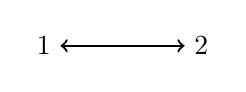
\begin{tikzpicture}
\node (atom4) at (0,0) {1};
\node (atom5) at (2,0) {2};
\draw[<->, thick] (atom4)--(atom5);
\end{tikzpicture}
\end{center}}
\item $\forall x (\atom{R}{c,a} \eiff \atom{R}{x,a}), Rca \eiff \forall x\,\atom{R}{x,a}$ \hfill \myanswer{Not logically equivalent}
\\\myanswer{Counter-interpretation, consider the following diagram, allowing `$a$' to name 1 and `$c$' to name 2:
\begin{center}
\begin{tikzpicture}
\node (atom4) at (0,0) {1};
\node (atom5) at (2,0) {2};
\draw[->, thick] (atom4)+(-0.15,0.15) arc (-330:-30:.3); 
%\draw[->, thick] (atom5)+(0.15,-0.15) arc (-150:150:.3); 
%\draw[<->, thick] (atom4)--(atom5);
\end{tikzpicture}
\end{center}}
\end{earg}

\solutions
\problempart
\label{pr.FOLvalidornot}
For each of the following arguments: If it is valid in FOL, give a proof. If it is invalid, construct an interpretation to show that it is invalid.
\begin{earg}
\item $\exists y\forall x\,\atom{R}{x,y} \therefore \forall x\exists y\,\atom{R}{x,y}$ \hfill \myanswer{Valid
\begin{fitchproof}
\hypo{EAr}{\exists y \forall x\,\atom{R}{x,y}}
\open
	\hypo{Ar}{\forall x\,\atom{R}{x,a}}
	\have{r}{\atom{R}{b,a}}\Ae{Ar}
	\have{Er}{\exists y\,\atom{R}{b,y}}\Ei{r}
\close
\have{Er1}{\exists y\,\atom{R}{b,y}}\Ee{EAr, Ar-Er}
\have{AEr}{\forall x \exists y\,\atom{R}{x,y}}\Ai{Er1}
\end{fitchproof}}
\item $\forall x\exists y\,\atom{R}{x,y} \therefore  \exists y\forall x\,\atom{R}{x,y}$ \hfill \myanswer{Not valid
\\Counter interpretation: let the domain be the numbers $1$ and $2$. Let `$Rxy$' be true of $1$ and $2$, and of $2$ and $1$ (but not $1$ and itself or $2$ and itself).}
\item $\exists x(\atom{P}{x} \eand \enot \atom{Q}{x}) \therefore \forall x(\atom{P}{x} \eif \enot \atom{Q}{x})$ \hfill \myanswer{Not valid
\\Counter interpretation: let the domain be the numbers $1$ and $2$. Let `$Px$' be true of everything in the domain. Let `$Qx$' be true of, and only of, $2$.}
\item $\forall x(\atom{S}{x} \eif \atom{T}{a}), \atom{S}{d} \therefore \atom{T}{a}$ \hfill \myanswer{Valid
\begin{fitchproof}
\hypo{Ast}{\forall x (\atom{S}{x} \eif \atom{T}{a})}
\hypo{s}{\atom{S}{d}}
\have{st}{\atom{S}{d} \eif \atom{T}{a}}\Ae{Ast}
\have{t}{\atom{T}{a}}\ce{st, s}
\end{fitchproof}}
\item $\forall x(Ax\eif \atom{B}{x}), \forall x(\atom{B}{x} \eif \atom{C}{x}) \therefore \forall x(\atom{A}{x} \eif \atom{C}{x})$ \hfill \myanswer{Valid
\begin{fitchproof}
\hypo{Aab}{\forall x (\atom{A}{x} \eif \atom{B}{x})}
\hypo{Abc}{\forall x (\atom{B}{x} \eif \atom{C}{x})}
\have{ab}{\atom{A}{a} \eif \atom{B}{a}}\Ae{Aab}
\have{bc}{\atom{B}{a} \eif \atom{C}{a}}\Ae{Abc}
\open
	\hypo{a}{\atom{A}{a}}
	\have{b}{\atom{B}{a}}\ce{ab, a}
	\have{c}{\atom{C}{a}}\ce{bc, b}
\close
\have{ac}{\atom{A}{a} \eif \atom{C}{a}}\ci{a-c}
\have{Aac}{\forall x (\atom{A}{x} \eif \atom{C}{x})}\Ai{ac}
\end{fitchproof}}
\item $\exists x(\atom{D}{x} \eor \atom{E}{x}), \forall x(\atom{D}{x} \eif \atom{F}{x}) \therefore \exists x(\atom{D}{x} \eand \atom{F}{x})$ \hfill \myanswer{Invalid\\
Counter-interpretation: let the domain be the number $1$ . Let `$Dx$' hold of nothing. Let both `$Ex$' and `$Fx$' hold of everything.}
\item $\forall x\forall y(\atom{R}{x,y} \eor \atom{R}{y,x}) \therefore Rjj$ \hfill \myanswer{Valid
\begin{fitchproof}
\hypo{AArr}{\forall x \forall y (\atom{R}{x,y} \eor \atom{R}{y,x})}
\have{Arr}{\forall y (\atom{R}{j,y} \eor \atom{R}{y,j})}\Ae{AArr}
\have{rr}{\atom{R}{j,j} \eor \atom{R}{j,j}}\Ae{Arr}
\open
	\hypo{r1}{\atom{R}{j,j}}
	\have{r2}{\atom{R}{j,j}}\by{R}{r1}
\close
\open
	\hypo{r3}{\atom{R}{j,j}}
	\have{r4}{\atom{R}{j,j}}\by{R}{r3}
\close
\have{r5}{\atom{R}{j,j}}\oe{rr, r1-r2, r3-r4}
\end{fitchproof}}

\item $\exists x\exists y(\atom{R}{x,y} \eor \atom{R}{y,x}) \therefore Rjj$ \hfill \myanswer{Invalid\\
Counter-interpretation: consider the following diagram, allowing `$j$' to name $2$.
\begin{center}
\begin{tikzpicture}
\node (atom4) at (0,0) {1};
\node (atom5) at (2,0) {2};
\draw[->, thick] (atom4)+(-0.15,0.15) arc (-330:-30:.3); 
%\draw[->, thick] (atom5)+(0.15,-0.15) arc (-150:150:.3); 
%\draw[<->, thick] (atom4)--(atom5);
\end{tikzpicture}
\end{center}}
\item $\forall x\,\atom{P}{x} \eif \forall x\,\atom{Q}{x}, \exists x \enot \atom{P}{x} \therefore \exists x \enot \atom{Q}{x}$ \hfill \myanswer{Invalid\\
Counter-interpretation: let the domain be the number $1$. Let `$Px$' be true of nothing. Let `$Qx$' be true of everything.}

\item $\exists x\,\atom{M}{x} \eif \exists x\,\atom{N}{x}$, $\enot \exists x\,\atom{N}{x}\therefore  \forall x \enot \atom{M}{x}$\hfill \myanswer{Valid\\
\begin{fitchproof}
\hypo{EMiEN}{\exists x\,\atom{M}{x} \eif \exists x\,\atom{N}{x}}
\hypo{nEN}{\enot \exists x\,\atom{N}{x}}
\open
  \hypo{Ma}{\atom{M}{a}}
  \have{EM}{\exists x\,\atom{M}{x}}\Ei{Ma}
  \have{EN}{\exists x\,\atom{N}{x}}\ce{EMiEN,EM}
  \have{abs}{\ered}\ri{EN, nEN}
\close
\have{nMa}{\enot \atom{M}{a}}\ni{Ma-abs}
\have{AnM}{\forall x \enot \atom{M}{x}}\Ai{nMa}
\end{fitchproof}}
\end{earg}

\stepcounter{chapter}
\chapter{Conversion of quantifiers}\setcounter{ProbPart}{0}
\problempart
Show in each case that the sentences are provably inconsistent:
\begin{earg}
\item $Sa\eif \atom{T}{m}, \atom{T}{m} \eif \atom{S}{a}, \atom{T}{m} \eand \enot \atom{S}{a}$
\myanswer{\begin{fitchproof}
\hypo{st}{\atom{S}{a} \eif \atom{T}{m}}
\hypo{ts}{\atom{T}{m} \eif \atom{S}{a}}
\hypo{tns}{\atom{T}{m} \eand \enot \atom{S}{a}}
\have{t}{\atom{T}{m}}\ae{tns}
\have{ns}{\enot \atom{S}{a}}\ae{tns}
\have{s}{\atom{S}{a}}\ce{ts, t}
\have{red}{\ered}\ri{ns,s}
\end{fitchproof}}
\item $\enot\exists x\,\atom{R}{x,a}, \forall x \forall y\,\atom{R}{y,x}$
\myanswer{\begin{fitchproof}
\hypo{nEr}{\enot \exists x\,\atom{R}{x,a}}
\hypo{AAr}{\forall x \forall y\,\atom{R}{y,x}}
\have{Anr}{\forall x \enot \atom{R}{x,a}}\cq{nEr}
\have{nr}{\enot \atom{R}{b,a}}\Ae{Anr}
\have{Ar}{\forall y\,\atom{R}{y,a}}\Ae{AAr}
\have{r}{\atom{R}{b,a}}\Ae{Ar}
\have{red}{\ered}\ri{r, nr}
\end{fitchproof}}
\item $\enot\exists x \exists y\,\atom{L}{x,y}, \atom{L}{a,a}$
\myanswer{\begin{fitchproof}
\hypo{nEEl}{\enot \exists x \exists y\,\atom{L}{x,y}}
\hypo{l}{\atom{L}{a,a}}
\have{AnEl}{\forall x \enot \exists y\,\atom{L}{x,y}}\cq{nEEl}
\have{nEl}{\enot \exists y\,\atom{L}{a,y}}\Ae{AnEl}
\have{Anl}{\forall y \enot \atom{L}{a,y}}\cq{nEl}
\have{n}{\enot \atom{L}{a,a}}\Ae{Anl}
\have{red}{\ered}\ri{l,n}
\end{fitchproof}}
\item $\forall x(\atom{P}{x} \eif \atom{Q}{x}), \forall z(\atom{P}{z} \eif \atom{R}{z}), \forall y\,\atom{P}{y}, \enot \atom{Q}{a} \eand \enot \atom{R}{b}$
\myanswer{\begin{fitchproof}
\hypo{Apq}{\forall x(\atom{P}{x} \eif \atom{Q}{x})}
\hypo{Apr}{\forall z(\atom{P}{z} \eif \atom{R}{z})}
\hypo{Ap}{\forall y\,\atom{P}{y}}
\hypo{nqnr}{\enot \atom{Q}{a} \eand \enot \atom{R}{b}}
\have{nq}{\enot \atom{Q}{a}}\ae{nqnr}
\have{pq}{\atom{P}{a} \eif \atom{Q}{a}}\Ae{Apq}
\have{np}{\enot \atom{P}{a}}\mt{pq, nq}
\have{p}{\atom{P}{a}}\Ae{Ap}
\have{red}{\ered}\ri{p,np}
\end{fitchproof}}
\end{earg}

\problempart
Show that each pair of sentences is provably equivalent: %TB: Again, have to do some manual numbering to make the multicols have enough space.

\

1.  $\forall x (Ax\eif \enot \atom{B}{x}), \enot\exists x(\atom{A}{x} \eand \atom{B}{x})$
\myanswer{\begin{multicols}{2}
\begin{fitchproof}
\hypo{Aanb}{\forall x (\atom{A}{x} \eif \enot \atom{B}{x})}
\open
	\hypo{Eab}{\exists x (\atom{A}{x} \eand \atom{B}{x})}
	\open
		\hypo{ab}{\atom{A}{a} \eand \atom{B}{a}}
		\have{a}{\atom{A}{a}}\ae{ab}
		\have{b}{\atom{B}{a}}\ae{ab}
		\have{anb}{\atom{A}{a} \eif \enot \atom{B}{a}}\Ae{Aanb}
		\have{nb}{\enot \atom{B}{a}}\ce{anb, a}
		\have{red}{\ered}\ri{b, nb}
	\close
	\have{red1}{\ered}\Ee{Eab, ab-red}
	\close
\have{nEab}{\enot \exists x(\atom{A}{x} \eand \atom{B}{x})}\ni{Eab-red1}
\end{fitchproof}
\begin{fitchproof}
\hypo{nEab}{\enot \exists x(\atom{A}{x} \eand \atom{B}{x})}
\have{Anab}{\forall x\enot(\atom{A}{x} \eand \atom{B}{x})}\cq{nEab}
\have{nab}{\enot (\atom{A}{a} \eand \atom{B}{a})}\Ae{Anab}
\open
	\hypo{a}{\atom{A}{a}}
	\open
		\hypo{b}{\atom{B}{a}}
		\have{ab}{\atom{A}{a} \eand \atom{B}{a}}\ai{a,b}
		\have{red}{\ered}\ri{ab,nab}
	\close
	\have{nb}{\enot \atom{B}{a}}\ni{b-red}
\close
\have{anb}{\atom{A}{a} \eif \enot \atom{B}{a}}\ci{a-nb}
\have{Aanb}{\forall x (\atom{A}{x} \eif \enot \atom{B}{x})}\Ai{anb}		
\end{fitchproof}
\end{multicols}}
2. $\forall x (\enot \atom{A}{x}\eif \atom{B}{d}), \forall x\,\atom{A}{x} \eor \atom{B}{d}$
\myanswer{\begin{multicols}{2}
\begin{fitchproof}
\hypo{Anab}{\forall x(\enot \atom{A}{x} \eif \atom{B}{d})}
\have{nab}{\enot \atom{A}{a} \eif \atom{B}{d}}\Ae{Anab}
\open
	\hypo{b}{\atom{B}{d}}
	\have{Aab}{\forall x\,\atom{A}{x} \eor \atom{B}{d}}\oi{ab}
\close
\open
	\hypo{nb}{\enot \atom{B}{d}}
	\have{nna}{\enot \enot \atom{A}{a}}\mt{nab, nb}
	\have{a}{\atom{A}{a}}\dne{nna}
	\have{Aa}{\forall x\,\atom{A}{x}}\Ae{a}
	\have{Aab1}{\forall x\,\atom{A}{x} \eor \atom{B}{d}}\oi{Aa}
\close
\have{Aab2}{\forall xAx \eor \atom{B}{d}}\tnd{b-Aab, nb-Aab1}
\end{fitchproof}
\begin{fitchproof}
\hypo{Aab}{\forall x\,\atom{A}{x} \eor \atom{B}{d}}
\open
	\hypo{na}{\enot \atom{A}{a}}
	\open
		\hypo{Aa}{\forall x\,\atom{A}{x}}
		\have{a}{\atom{A}{a}}\Ae{Aa}
		\have{red}{\ered}\ri{a, na}
	\close
	\have{nAa}{\enot \forall x\,\atom{A}{x}}\ni{Aa-red}
	\have{b}{\atom{B}{d}}\ds{Aab, nAa}
\close
\have{nab}{\enot \atom{A}{a} \eif \atom{B}{d}}\ci{na-b}
\have{Anab}{\forall x (\atom{A}{x} \eif \atom{B}{d})}\Ai{nab}
\end{fitchproof}
\end{multicols}}


\problempart
In \S\ref{s:MoreMonadic}, we considered what happens when we move quantifiers `across' various logical operators. Show that each pair of sentences is provably equivalent: %TB: Again, manual line numbering to give multicols enough space.

\

1.  $\forall x (\atom{F}{x} \eand \atom{G}{a}), \forall x\,\atom{F}{x} \eand \atom{G}{a}$ 
\myanswer{
\begin{multicols}{2}
\begin{fitchproof}
\hypo{Afg}{\forall x (\atom{F}{x} \eand \atom{G}{a})}
\have{fg}{\atom{F}{b} \eand \atom{G}{a}}\Ae{Afg}
\have{f}{\atom{F}{b}}\ae{fg}
\have{g}{\atom{G}{a}}\ae{ga}
\have{Af}{\forall x\,\atom{F}{x}}\Ai{f}
\have{Afg1}{\forall x\,\atom{F}{x} \eand \atom{G}{a}}\ai{Af, g}
\end{fitchproof}
\begin{fitchproof}
\hypo{Afg}{\forall x\,\atom{F}{x} \eand \atom{G}{a}}
\have{Af}{\forall x\,\atom{F}{x}}\ae{Afg}
\have{g}{\atom{G}{a}}\ae{Afg}
\have{f}{\atom{F}{b}}\Ae{Af}
\have{fg}{\atom{F}{b} \eand \atom{G}{a}}\ai{f, g}
\have{Afg1}{\forall x (\atom{F}{x} \eand \atom{G}{a})}\Ai{fg}
\end{fitchproof}
\end{multicols}}
2. $\exists x (\atom{F}{x} \eor \atom{G}{a}), \exists x\,\atom{F}{x} \eor \atom{G}{a}$
\myanswer{
\begin{multicols}{2}
\begin{fitchproof}
\hypo{Efg}{\exists x (\atom{F}{x} \eor \atom{G}{a})}
\open
	\hypo{fg}{\atom{F}{b} \eor \atom{G}{a}}
	\open
		\hypo{f}{\atom{F}{b}}
		\have{Ef}{\exists x\,\atom{F}{x}}\Ei{f}
		\have{Efg1}{\exists x\,\atom{F}{x} \eor \atom{G}{a}}\oi{Ef}
	\close
	\open
		\hypo{g}{\atom{G}{a}}
		\have{Efg2}{\exists x\,\atom{F}{x} \eor \atom{G}{a}}\oi{g}
	\close		
	\have{Efg3}{\exists x\,\atom{F}{x} \eor \atom{G}{a}}\oe{fg, f-Efg1, g-Efg2}
\close
\have{Efg4}{\exists x\,\atom{F}{x} \eor \atom{G}{a}}\Ee{Efg, fg-Efg3}
\end{fitchproof}
\begin{fitchproof}
\hypo{Efg}{\exists x\,\atom{F}{x} \eor \atom{G}{a}}
\open
	\hypo{Ef}{\exists x\,\atom{F}{x}}
	\open
		\hypo{f}{\atom{F}{b}}
		\have{fg}{\atom{F}{b} \eor \atom{G}{a}}\oi{f}
		\have{Efg1}{\exists x (\atom{F}{x} \eor \atom{G}{a})}\Ei{fg}
	\close
	\have{Efg2}{\exists x (\atom{F}{x} \eor \atom{G}{a})}\Ee{Ef, f-Efg1}
\close
\open
	\hypo{g}{\atom{G}{a}}
	\have{fbg}{\atom{F}{b} \eor \atom{G}{a}}\oi{g}
	\have{Efg3}{\exists x (\atom{F}{x} \eor \atom{G}{a})}\Ei{fbg}
\close
\have{Efg4}{\exists x (\atom{F}{x} \eor \atom{G}{a})}\oe{Efg, Ef-Efg2, g-Efg3}
\end{fitchproof}
\end{multicols}}
3. $\forall x(\atom{G}{a} \eif \atom{F}{x}), \atom{G}{a} \eif \forall x\,\atom{F}{x}$
\myanswer{\begin{multicols}{2}
\begin{fitchproof}
\hypo{Agf}{\forall x(\atom{G}{a} \eif \atom{F}{x})}
\have{gf}{\atom{G}{a} \eif \atom{F}{b}}\Ae{Agf}
\open
	\hypo{g}{\atom{G}{a}}
	\have{f}{\atom{F}{b}}\ce{gf, g}
	\have{Af}{\forall x\,\atom{F}{x}}\Ai{f}
\close
\have{gAf}{\atom{G}{a} \eif \forall x\,\atom{F}{x}}\ci{g-Af}
\end{fitchproof}
\begin{fitchproof}
\hypo{gAf}{\atom{G}{a} \eif \forall x\,\atom{F}{x}}
\open
	\hypo{g}{\atom{G}{a}}
	\have{Af}{\forall x\,\atom{F}{x}}\ce{gAf, g}
	\have{f}{\atom{F}{b}}\Ae{Af}
\close
\have{gf}{\atom{G}{a} \eif \atom{F}{b}}\ci{g-f}
\have{Agf}{\forall x (\atom{G}{a} \eif \atom{F}{x})}\Ai{gf}
\end{fitchproof}
\end{multicols}}

4. $\forall x(\atom{F}{x} \eif \atom{G}{a}), \exists x\,\atom{F}{x} \eif \atom{G}{a}$
\myanswer{\begin{multicols}{2}
\begin{fitchproof}
\hypo{Afg}{\forall x(\atom{F}{x} \eif \atom{G}{a})}
\open
	\hypo{Ef}{\exists x\,\atom{F}{x}}
	\open
		\hypo{f}{\atom{F}{b}}
		\have{fg}{\atom{F}{b} \eif \atom{G}{a}}\Ae{Afg}
		\have{g}{\atom{G}{a}}\ce{fg, f}
	\close
	\have{g1}{\atom{G}{a}}\Ee{Ef, f-g}
\close
\have{Efg}{\exists x\,\atom{F}{x} \eif \atom{G}{a}}\ci{Ef-g1}	
\end{fitchproof}
\begin{fitchproof}
\hypo{Efg}{\exists x\,\atom{F}{x} \eif \atom{G}{a}}
\open
	\hypo{f}{\atom{F}{b}}
	\have{Ef}{\exists x\,\atom{F}{x}}\Ei{f}
	\have{g}{\atom{G}{a}}\ce{Efg,Ef}
\close
\have{fg}{\atom{F}{b} \eif \atom{G}{a}}\ci{f-g}
\have{Afg}{\forall x(\atom{F}{x} \eif \atom{G}{a})}\Ai{fg}	
\end{fitchproof}
\end{multicols}}
5. $\exists x(\atom{G}{a} \eif \atom{F}{x}), \atom{G}{a} \eif \exists x\,\atom{F}{x}$
\myanswer{\begin{multicols}{2}
\begin{fitchproof}
\hypo{Egf}{\exists x(\atom{G}{a} \eif \atom{F}{x})}
\open
	\hypo{g}{\atom{G}{a}}
	\open
		\hypo{gf}{\atom{G}{a} \eif \atom{F}{b}}
		\have{f}{\atom{F}{b}}\ce{gf, g}
		\have{Ef}{\exists x\,\atom{F}{x}}\Ei{f}
	\close
	\have{Ef1}{\exists x\,\atom{F}{x}}\Ee{Egf, gf-Ef}
\close
\have{gEf}{\atom{G}{a} \eif \exists x\,\atom{F}{x}}\ci{g-Ef1}
\end{fitchproof}
\begin{fitchproof}
\hypo{gEf}{\atom{G}{a} \eif \exists x\,\atom{F}{x}}
\open
	\hypo{g}{\atom{G}{a}}
	\have{Ef}{\exists x\,\atom{F}{x}}
	\open
		\hypo{f}{\atom{F}{b}}
		\open
			\hypo{g1}{\atom{G}{a}}
			\have{f1}{\atom{F}{b}}\by{R}{f}
		\close
		\have{gf}{\atom{G}{a} \eif \atom{F}{b}}\ci{g1-f1}
		\have{Egf}{\exists x(\atom{G}{a} \eif \atom{F}{x})}\Ei{gf}
	\close
	\have{Egf1}{\exists x (\atom{G}{a} \eif \atom{F}{x})}\Ee{Ef, f-Egf}
\close
\open
	\hypo{ng}{\enot \atom{G}{a}}
	\open
		\hypo{g2}{\atom{G}{a}}
		\have{red}{\ered}\ri{g2, ng}
		\have{f2}{\atom{F}{b}}\re{red}
	\close
	\have{gf1}{\atom{G}{a} \eif \atom{F}{b}}\ce{g2-f2}
	\have{Egf2}{\exists x (\atom{G}{a} \eif \atom{F}{x})}\Ei{gf1}
\close
\have{con}{\exists x (\atom{G}{a} \eif \atom{F}{x})}\tnd{g-Egf1, ng-Egf2}
\end{fitchproof}
\end{multicols}}

6. $\exists x(\atom{F}{x} \eif \atom{G}{a}), \forall x\,\atom{F}{x} \eif \atom{G}{a}$
\myanswer{\begin{multicols}{2}
\begin{fitchproof}
\hypo{Efg}{\exists x (\atom{F}{x} \eif \atom{G}{a})}
\open
	\hypo{Af}{\forall x\,\atom{F}{x}}
	\open
		\hypo{fg}{\atom{F}{b} \eif \atom{G}{a}}
		\have{f}{\atom{F}{b}}\Ae{Af}
		\have{g}{\atom{G}{a}}\ce{fg,f}
	\close
	\have{g1}{\atom{G}{a}}\Ee{Efg, fg-g}
\close
\have{Afg}{\forall x\,\atom{F}{x} \eif \atom{G}{a}}\ci{Af-g1}
\end{fitchproof}
\begin{fitchproof}
\hypo{Afg}{\forall x\,\atom{F}{x} \eif \atom{G}{a}}
\open
	\hypo{Af}{\forall x\,\atom{F}{x}}
	\have{g}{\atom{G}{a}}\ce{Afg, Af}
	\open
		\hypo{f}{\atom{F}{b}}
		\have{g1}{\atom{G}{a}}\by{R}{g}
	\close
	\have{fg}{\atom{F}{b} \eif \atom{G}{a}}\ci{f-g1}
	\have{Efg}{\exists x (\atom{F}{x} \eif \atom{G}{a})}\Ei{fg}
\close
\open
	\hypo{nAf}{\enot \forall x\,\atom{F}{x}}
	\have{Enf}{\exists x \enot \atom{F}{x}}\cq{nAf}
	\open
		\hypo{nf}{\enot \atom{F}{b}}
		\open
			\hypo{f1}{\atom{F}{b}}
			\have{red}{\ered}\ri{f1, nf}
			\have{g2}{\atom{G}{a}}\re{red}
		\close
		\have{fg1}{\atom{F}{b} \eif \atom{G}{a}}\ci{f1-g2}
		\have{Efg1}{\exists x (\atom{F}{x} \eif \atom{G}{a})}\Ei{fg1}
	\close
	\have{Efg2}{\exists x (\atom{F}{x} \eif \atom{G}{a})}\Ee{Enf, nf-Efg1}
\close
\have{Efg3}{\exists x (\atom{F}{x} \eif \atom{G}{a})}\tnd{Af-Efg, nAf-Efg2}
\end{fitchproof}
\end{multicols}}
NB: the variable `$x$' does not occur in `$\atom{G}{a}$'. When all the quantifiers occur at the beginning of a sentence, that sentence is said to be in \emph{prenex normal form}. Together with the CQ rules, these equivalences are sometimes called \emph{prenexing rules}, since they give us a means for putting any sentence into prenex normal form.

\chapter{Rules for identity}\setcounter{ProbPart}{0}
\problempart
\label{pr.identity}
Provide a proof of each claim.
\begin{earg}
\item $Pa \eor \atom{Q}{b}, \atom{Q}{b} \eif b=c, \enot \atom{P}{a} \proves \atom{Q}{c}$
\myanswer{
\begin{fitchproof}
\hypo{pq}{\atom{P}{a} \eor \atom{Q}{b}}
\hypo{qbi}{\atom{Q}{b} \eif b=c}
\hypo{np}{\enot \atom{P}{a}}
\have{q}{\atom{Q}{b}}\ds{pq, np}
\have{i}{b=c}\ce{qbi, q}
\have{qc}{\atom{Q}{c}}\ie{i,q}
\end{fitchproof}}
\item $m=n \eor n=o, \atom{A}{n} \proves \atom{A}{m} \eor \atom{A}{o}$
\myanswer{
\begin{fitchproof}
\hypo{mnino}{m=n \eor n=o}
\hypo{an}{\atom{A}{n}}
\open
	\hypo{min}{m=n}
	\have{am}{\atom{A}{m}}\ie{min, an}
	\have{amao}{\atom{A}{m} \eor \atom{A}{o}}\oi{am}
\close
\open
	\hypo{nio}{n=o}
	\have{ao}{\atom{A}{o}}\ie{nio, ao}
	\have{amao1}{\atom{A}{m} \eor \atom{A}{o}}\oi{ao}
\close
\have{amao2}{\atom{A}{m} \eor \atom{A}{o}}\oe{mnino, min-amao, nio-amao1}
\end{fitchproof}}
\item $\forall x\ x=m, \atom{R}{m,a} \proves \exists x\,\atom{R}{x,x}$
\myanswer{\begin{fitchproof}
\hypo{Axim}{\forall x\ x=m}
\hypo{rma}{\atom{R}{m,a}}
\have{aim}{a=m}\Ae{Axim}
\have{raa}{\atom{R}{a,a}}\ie{aim, rma}
\have{Erxx}{\exists x\,\atom{R}{x,x}}\Ei{raa}
\end{fitchproof}}
\item $\forall x\forall y(\atom{R}{x,y} \eif x=y)\proves \atom{R}{a,b} \eif \atom{R}{b,a}$
\myanswer{\begin{fitchproof}
\hypo{AArxiy}{\forall x \forall y(\atom{R}{x,y} \eif x = y)}
\open
	\hypo{rab}{\atom{R}{a,b}}
	\have{Araiy}{\forall y(\atom{R}{a,y} \eif a = y)}\Ae{AArxiy}
	\have{raib}{\atom{R}{a,b} \eif a=b}\Ae{Araiy}
	\have{aib}{a=b}\ce{raib, rab}
	\have{raa}{\atom{R}{a,a}}\ie{aib, rab}
	\have{rba}{\atom{R}{b,a}}\ie{aib, raa}
\close
\have{rabrba}{\atom{R}{a,b} \eif \atom{R}{b,a}}\ci{rab-rba}
\end{fitchproof}}
\item $\enot \exists x\enot x = m \proves \forall x\forall y (\atom{P}{x} \eif \atom{P}{y})$
\myanswer{\begin{fitchproof}
\hypo{nEnxim}{\enot \exists x \enot x = m}
\have{Annxim}{\forall x \enot \enot x =m}\cq{nEnxim}
\have{nnaim}{\enot \enot a = m}\Ae{Annxim}
\have{aim}{a = m}\dne{nnaim}
\have{nnbim}{\enot \enot b = m}\Ae{Annxim}
\have{bim}{b = m}\dne{nnbim}
\open
	\hypo{pa}{\atom{P}{a}}
	\have{pm}{\atom{P}{m}}\ie{nnaim, pa}
	\have{pb}{\atom{P}{b}}\ie{nnbim, pm}
\close
\have{papb}{\atom{P}{a} \eif \atom{P}{b}}\ci{pa-pb}
\have{Apapy}{\forall y (\atom{P}{a} \eif \atom{P}{y})}\Ai{papb}
\have{AApxpy}{\forall x\forall y (\atom{P}{x} \eif \atom{P}{y})}\Ai{Apapy}
\end{fitchproof}}
\item $\exists x\,\atom{J}{x}, \exists x \enot \atom{J}{x}\proves \exists x \exists y\ \enot x = y$
\myanswer{\begin{fitchproof}
\hypo{Ej}{\exists x\,\atom{J}{x}}
\hypo{Enj}{\exists x \enot \atom{J}{x}}
\open
	\hypo{j}{\atom{J}{a}}
	\open
		\hypo{nj}{\enot \atom{J}{b}}
		\open
			\hypo{aib}{a=b}
			\have{jb}{\atom{J}{b}}\ie{aib, j}
			\have{red}{\ered}\ri{jb, nj}
		\close
		\have{naib}{\enot a = b}\ni{aib-red}
		\have{Enaiy}{\exists y \enot a = y}\Ei{naib}
		\have{EEnxiy}{\exists x \exists y \enot x = y}\Ei{Enaiy}
	\close
	\have{EEnxiy1}{\exists x \exists y \enot x = y}\Ee{Enj, nj-EEnxiy}
\close
\have{EEnxiy2}{\exists x \exists y \enot x = y}\Ee{Ej, j-EEnxiy1}
\end{fitchproof}}

\item $\forall x(x=n \eiff \atom{M}{x}), \forall x(\atom{O}{x} \eor \enot \atom{M}{x})\proves \atom{O}{n}$
\myanswer{\begin{fitchproof}
\hypo{Axinm}{\forall x(x = n \eiff \atom{M}{x})}
\hypo{Aonm}{\forall x(\atom{O}{x} \eor \enot \atom{M}{x})}
\have{ninm}{n = n \eiff \atom{M}{n}}\Ae{Axinm}
\have{nin}{n=n}\ii{}
\have{m}{\atom{M}{n}}\be{ninm,nin}
\have{onm}{\atom{O}{n} \eor \enot \atom{M}{n}}\Ae{Aonm}
\open
	\hypo{no}{\enot \atom{O}{n}}
	\have{nm}{\enot \atom{M}{n}}\ds{onm, no}
	\have{red}{\ered}\ri{m, nm}
\close
\have{nno}{\enot\enot \atom{O}{n}}\ni{no-red}
\have{o}{\atom{O}{n}}\dne{nno}
\end{fitchproof}}

\item $\exists x\,\atom{D}{x}, \forall x(x=p \eiff \atom{D}{x})\proves \atom{D}{p}$
\myanswer{\begin{fitchproof}
\hypo{Ed}{\exists x\,\atom{D}{x}}
\hypo{Axd}{\forall x(x = p \eiff \atom{D}{x})}
\open
	\hypo{d}{\atom{D}{c}}
	\have{cipd}{c = p \eiff \atom{D}{c}}\Ae{Axd}
	\have{cip}{c = p}\be{cipd, d}
	\have{dp}{\atom{D}{p}}\ie{cip, d}
\close
\have{dp1}{\atom{D}{p}}\Ee{Ed, d-dp}
\end{fitchproof}}

\item $\exists x\bigl[(\atom{K}{x} \eand \forall y(\atom{K}{y} \eif x=y)) \eand \atom{B}{x}\bigr], \atom{K}{d} \proves \atom{B}{d}$
\myanswer{\begin{fitchproof}
\hypo{EkAkb}{\exists x\bigl[(\atom{K}{x} \eand \forall y(\atom{K}{y} \eif x=y) \eand \atom{B}{x}\bigr]}
\hypo{kd}{\atom{K}{d}}
\open
	\hypo{kAkb}{(\atom{K}{a} \eand \forall y(\atom{K}{y} \eif a=y)) \eand \atom{B}{a}}
	\have{kAk}{\atom{K}{a} \eand \forall y(\atom{K}{y} \eif a=y)}\ae{kAkb}
	\have{k}{\atom{K}{a}}\ae{kAk}
	\have{Ak}{\forall y (\atom{K}{y} \eif a = y)}\ae{kAk}
	\have{kdaid}{\atom{K}{d} \eif a = d}\Ae{Ak}
	\have{aid}{a = d}\ce{kdaid, kd}
	\have{b}{\atom{B}{a}}\ae{kAkb}
	\have{bd}{\atom{B}{d}}\ie{aid, b}
\close
\have{con}{\atom{B}{d}}\Ee{EkAkb, kAkb-bd}
\end{fitchproof}}

\item $\proves \atom{P}{a} \eif \forall x(\atom{P}{x} \eor \enot x = a)$
\myanswer{\begin{fitchproof}
\open
	\hypo{pa}{\atom{P}{a}}
	\open
		\hypo{bia}{b = a}
		\have{pb}{\atom{P}{b}}\ie{bia, pa}
		\have{pboi}{\atom{P}{b} \eor \enot b = a}\oi{pb}
	\close
	\open
		\hypo{nbia}{\enot b = a}
		\have{pboi1}{\atom{P}{b} \eor \enot b = a}\oi{nbia}
	\close
	\have{pboi2}{\atom{P}{b} \eor \enot b = a}\tnd{bia-pboi, nbia-pboi1}
	\have{Apoi}{\forall x (\atom{P}{x} \eor \enot x = a)}\Ai{pboi2}
\close
\have{con}{\atom{P}{a} \eif \forall x (\atom{P}{x} \eor \enot x = a)}\ci{pa-Apoi}
\end{fitchproof}}
\end{earg}

\problempart
Show that the following are provably equivalent:
\begin{ebullet}
\item $\exists x \bigl([\atom{F}{x} \eand \forall y (\atom{F}{y} \eif x = y)] \eand x = n\bigr)$
\item $\atom{F}{n} \eand \forall y (\atom{F}{y} \eif n= y)$
\end{ebullet}
And hence that both have a decent claim to symbolize the English sentence `Nick is the F'.
\\\myanswer{In one direction:
\begin{fitchproof}
\hypo{prem}{\exists x \bigl([\atom{F}{x} \eand \forall y (\atom{F}{y} \eif x = y)] \eand x = n\bigr)}
\open
	\hypo{prema}{{}[\atom{F}{a} \eand \forall y (\atom{F}{y} \eif a = y)] \eand a = n}
	\have{preman}{a = n}\ae{prema}
	\have{prema1}{\atom{F}{a} \eand \forall y (\atom{F}{y} \eif a = y)}\ae{prema}
	\have{prema2}{\atom{F}{a}}\ae{prema1}
	\have{fn}{\atom{F}{n}}\ie{preman, prema2}
	\have{prema3}{\forall y (\atom{F}{y} \eif a = y)}\ae{prema1}
	\have{prema4}{\forall y (\atom{F}{y} \eif n = y)}\ie{preman, prema3}
	\have{con1}{\atom{F}{n} \eand \forall y (\atom{F}{y} \eif n= y)}\ai{fn, prema4}
\close
\have{con}{\atom{F}{n} \eand \forall y (\atom{F}{y} \eif n= y)}\Ee{prem, prema-con1}
\end{fitchproof}\\And now in the other:
\begin{fitchproof}
\hypo{prem}{\atom{F}{n} \eand \forall y (\atom{F}{y} \eif n= y)}
\have{nin}{n = n}\ii{}
\have{near}{{}[\atom{F}{n} \eand \forall y (\atom{F}{y} \eif n= y)] \eand n = n}\ai{prem, nin}
\have{con}{\exists x \bigl([\atom{F}{x} \eand \forall y (\atom{F}{y} \eif x = y)] \eand x = n\bigr)}\Ei{near}
\end{fitchproof}}

\

\problempart
In \S\ref{sec.identity}, we claimed that the following are logically equivalent symbolizations of the English sentence `there is exactly one F':
\begin{ebullet}
\item $\exists x\,\atom{F}{x} \eand \forall x \forall y \bigl[(\atom{F}{x} \eand \atom{F}{y}) \eif x = y\bigr]$
\item $\exists x \bigl[\atom{F}{x} \eand \forall y (\atom{F}{y} \eif x = y)\bigr]$
\item $\exists x \forall y (\atom{F}{y} \eiff x = y)$
\end{ebullet}
Show that they are all provably equivalent. (\emph{Hint}: to show that three claims are provably equivalent, it suffices to show that the first proves the second, the second proves the third and the third proves the first; think about why.)\\
\myanswer{It suffices to show that the first proves the second, the second proves the third and the third proves the first, for we can then show that any of them prove any others, just by chaining the proofs together (numbering lines, where necessary. Armed with this, we start on the first proof:
\begin{fitchproof}
\hypo{prem}{\exists x\,\atom{F}{x} \eand \forall x \forall y \bigl[(\atom{F}{x} \eand \atom{F}{y}) \eif x = y\bigr]}
\have{prem1}{\exists x\,\atom{F}{x}}\ae{prem}
\have{prem2}{\forall x \forall y \bigl[(\atom{F}{x} \eand \atom{F}{y}) \eif x = y\bigr]}\ae{prem}
\open
	\hypo{fa}{\atom{F}{a}}
	\have{prem2a}{\forall y \bigl[(\atom{F}{a} \eand \atom{F}{y}) \eif a = y\bigr]}\Ae{prem2}
	\have{prem2b}{(\atom{F}{a} \eand \atom{F}{b}) \eif a = b}\Ae{prem2a}
	\open
		\hypo{fb}{\atom{F}{b}}
		\have{fafb}{\atom{F}{a} \eand \atom{F}{b}}\ai{fa, fb}
		\have{aib}{a=b}\ce{prem2b, fafb}
	\close
	\have{fbaib}{\atom{F}{b} \eif a =b}\ci{fb-aib}
	\have{Afb}{\forall y(\atom{F}{y} \eif a =y)}\Ai{fbaib}	
	\have{cona}{\atom{F}{a} \eand \forall y(\atom{F}{y} \eif a = y))}\ai{fa, Afb}
	\have{con1}{\exists x \bigl[\atom{F}{x} \eand \forall y(\atom{F}{y} \eif x = y)\bigr]}\Ei{cona}
\close
\have{con}{\exists x \bigl[\atom{F}{x} \eand \forall y (\atom{F}{y} \eif x = y)\bigr]}\Ee{prem1, fa-con1}
\end{fitchproof}}

\
\\\myanswer{Now for the second proof:
\begin{fitchproof}
\hypo{prem}{\exists x \bigl[\atom{F}{x} \eand \forall y (\atom{F}{y} \eif x = y)\bigr]}
\open
	\hypo{prema}{\atom{F}{a} \eand \forall y (\atom{F}{y} \eif a = y)}
	\have{fa}{\atom{F}{a}}\ae{prema}
	\have{Af}{\forall y (\atom{F}{y} \eif a = y)}\ae{prema}
	\open
		\hypo{fb1}{\atom{F}{b}}
		\have{fbaib}{\atom{F}{b} \eif a = b}\Ae{Af}
		\have{aib1}{a = b}\ce{fbaib, fb1}
	\close
	\open
		\hypo{aib}{a = b}
		\have{fb}{\atom{F}{b}}\ie{aib, fa}
	\close
	\have{bic}{\atom{F}{b} \eiff a = b}\bi{fb1-aib1, aib-fb}
	\have{cony}{\forall y(\atom{F}{y} \eiff a = y)}\Ai{bic}
	\have{con1}{\exists x \forall y (\atom{F}{y} \eiff x = y)}\Ei{cony}
\close
\have{con}{\exists x \forall y (\atom{F}{y} \eiff x = y)}\Ee{prem, prema-con1}
\end{fitchproof}}

\noindent\myanswer{And finally, the third proof:
\begin{fitchproof}
\hypo{prem}{\exists x \forall y (\atom{F}{y} \eiff x = y)}
\open
	\hypo{prema}{\forall y(\atom{F}{y} \eiff a = y)}
	\have{premaa}{\atom{F}{a} \eiff a = a}\Ae{prema}
	\have{aia}{a = a}\ii{}
	\have{fa}{\atom{F}{a}}\be{premaa, aia}
	\have{Ef}{\exists x\,\atom{F}{x}}\Ei{fa}
	\open
		\hypo{fbfc}{\atom{F}{b} \eand \atom{F}{c}}
		\have{fb}{\atom{F}{b}}\ae{fbfc}
		\have{premab}{\atom{F}{b} \eiff a = b}\Ae{prema}
		\have{aib}{a = b}\be{premab, fb}
		\have{fc}{\atom{F}{c}}\ae{fbfc}
		\have{premac}{\atom{F}{c} \eiff a = c}\Ae{prema}
		\have{aic}{a = c}\be{premac, fc}
		\have{bic}{b = c}\ie{aib, aic}
	\close
	\have{nearbc}{(\atom{F}{b} \eand \atom{F}{c}) \eif b = c}\ci{fafb-bic}
	\have{nearb}{\forall y\bigl[(\atom{F}{b} \eand \atom{F}{y}) \eif b = y\bigr]}\Ai{nearbc}
	\have{near}{\forall x \forall y\bigl[(\atom{F}{x} \eand \atom{F}{y}) \eif x = y\bigr]}\Ai{nearb}
	\have{con1}{\exists x\,\atom{F}{x} \eand \forall x \forall y \bigl[(\atom{F}{x} \eand \atom{F}{y}) \eif x = y\bigr]}\ai{Ef, near}
\close
\have{con}{\exists x\,\atom{F}{x} \eand \forall x \forall y \bigl[(\atom{F}{x} \eand \atom{F}{y}) \eif x = y\bigr]}\Ee{prem, prema-con1}
\end{fitchproof}}


\
\problempart
Symbolize the following argument
	\begin{quote}
		There is exactly one F. There is exactly one G. Nothing is both F and G. So: there are exactly two things that are either F or G.
	\end{quote}
And offer a proof of it.\\
\myanswer{
\begin{earg}
\item $\exists x \bigl[\atom{F}{x} \eand \forall y (\atom{F}{y} \eif x = y)\bigr]$ 
\item $\exists x \bigl[\atom{G}{x} \eand \forall y ( \atom{G}{y} \eif x = y)\bigr]$
\item $\forall x (\enot \atom{F}{x} \eor \enot \atom{G}{x}) \therefore \phantom{.}$
\item[\therefore] $\exists x \exists y \bigl[\enot x = y \eand \forall z ((\atom{F}{z} \eor \atom{G}{z}) \eif (x = z \eor y = z))\bigr]$
\end{earg}}

\myanswer{\begin{fitchproof}
\hypo{p1}{\exists x \bigl[\atom{F}{x} \eand \forall y (\atom{F}{y} \eif x = y)\bigr]}
\hypo{p2}{\exists x \bigl[\atom{G}{x} \eand \forall y ( \atom{G}{y} \eif x = y)\bigr]}
\hypo{p3}{\forall x (\enot \atom{F}{x} \eor \enot \atom{G}{x})}
\open
	\hypo{p1a}{\atom{F}{a} \eand \forall y (\atom{F}{y} \eif a = y)}
	\have{fa}{\atom{F}{a}}\ae{p1a}
	\have{Afa}{\forall y (\atom{F}{y} \eif a = y)}\ae{p1a}
	\have{nfanga}{\enot \atom{F}{a} \eor \enot \atom{G}{a}}\Ae{p3}
	\have{nga}{\enot \atom{G}{a}}\ds{nfanga, fa}
	\open
		\hypo{p2b}{\atom{G}{b} \eand \forall y (\atom{G}{y} \eif b = y)}
		\have{gb}{\atom{G}{b}}\ae{p2b}
		\have{Agb}{\forall y (\atom{G}{y} \eif b = y)}\ae{p2b}
		\open
			\hypo{aib}{a = b}
			\have{ga}{\atom{G}{a}}\ie{aib, gb}
			\have{red}{\ered}\ri{ga, nga}
		\close
		\have{naib}{\enot a = b}\ni{aib-red}
		\open
			\hypo{fcorgc}{\atom{F}{c} \eor \atom{G}{c}}
			\open
				\hypo{fc}{\atom{F}{c}}
				\have{fcaic}{\atom{F}{c} \eif a = c}\Ae{Afa}
				\have{aic}{a = c}\ce{fcaic, fc}
				\have{aicbic}{a=c \eor b = c}\oi{aic}
			\close
			\open
				\hypo{gc}{\atom{G}{c}}
				\have{gcbic}{\atom{G}{c} \eif b = c}\Ae{Agb}
				\have{bic}{b = c}\ce{gcbic, gc}
				\have{aicbic1}{a=c \eor b = c}\oi{bic}
			\close
			\have{aicbic2}{a = c \eor b = c}\oe{fcorgc, fc-aicbic, gc-aicbic1}
		\close
		\have{nearabc}{(\atom{F}{c} \eor \atom{G}{c}) \eif (a = c \eor b = c)}\ci{fcorgc-aicbic2}
		\have{nearab}{\forall z ((\atom{F}{z} \eor \atom{G}{z}) \eif (a = z \eor b = z))}\Ai{nearabc}
		\have{conab}{\enot a = b \eand \forall z ((\atom{F}{z} \eor \atom{G}{z}) \eif (a = z \eor b = z))}\ai{naib, nearab}
		\have{cona}{\exists y\bigl[\enot a = y \eand \forall z ((\atom{F}{z} \eor \atom{G}{z}) \eif (a = z \eor y = z))\bigr]}\Ei{conab}
		\have{con2}{\exists x \exists y \bigl[\enot x = y \eand \forall z ((\atom{F}{z} \eor \atom{G}{z}) \eif (x = z \eor y = z))\bigr]}\Ei{cona}
	\close
	\have{con1}{\exists x \exists y \bigl[\enot x = y \eand \forall z ((\atom{F}{z} \eor \atom{G}{z}) \eif (x = z \eor y = z))\bigr]}\Ee{p2, p2b-con2}
\close
\have{con}{\exists x \exists y \bigl[\enot x = y \eand \forall z ((\atom{F}{z} \eor \atom{G}{z}) \eif (x = z \eor y = z))\bigr]}\Ee{p1, p1a-con1}
\end{fitchproof}}

\chapter{Derived rules}\setcounter{ProbPart}{0}
\problempart
Offer proofs which justify the addition of the second and fourth CQ rules as derived rules.\\
\myanswer{Justification for the second rule:
\begin{fitchproof}
	\hypo{nEa}{\enot \exists x\,\atom{A}{x}}
	\open
		\hypo{a}{\atom{A}{a}}
		\have{Ea}{\exists x\,\atom{A}{x}}\Ei{a}
		\have{red}{\ered}\ri{Ea, nEa}
	\close
	\have{na}{\enot \atom{A}{a}}\ni{a-red}
	\have{Ana}{\forall x \enot \atom{A}{x}}\Ai{na}
\end{fitchproof}}

\
\\
\myanswer{The fourth rule is harder to justify.  Here is a proof that
is relatively straightforward, but uses the derived rule DNE:
\begin{fitchproof}
\hypo{nAa}{\enot \forall x\,\atom{A}{x}}
  \open
  \hypo{nEna}{\enot \exists x \enot \atom{A}{x}}
    \open
    \hypo{na}{\enot \atom{A}{a}}
    \have{Ena}{\exists x \enot \atom{A}{x}}\Ei{na}
    \have{abs1}{\ered}\ri{Ena,nEna}
    \close
  \have{nna}{\enot \enot \atom{A}{a}}\ni{na-abs1}
  \have{a}{\atom{A}{a}}\dne{nna}
  \have{Aa}{\forall x\,\atom{A}{x}}\Ai{a}
  \have{abs2}{\ered}\ri{Aa,nAa}
  \close
\have{nnEna}{\enot \enot \exists x \enot \atom{A}{x}}\ni{nEna-abs2}
\have{Ena2}{\exists x \enot \atom{A}{x}}\dne{nnEna}
\end{fitchproof}\\
And here is a proof that does not use any derived rules:
\begin{fitchproof}
	\hypo{nAa}{\enot \forall x\,\atom{A}{x}} 
	\open
        \hypo{H1}{\exists x \enot \atom{A}{x}}
        \have{H1C}{\exists x \enot \atom{A}{x} \eand \exists x \enot \atom{A}{x}}\ai{H1}
        \have{conc1}{\exists x \enot \atom{A}{x}}\ae{H1C}
	\close
        \open
        \hypo{H2}{\enot \exists x \enot \atom{A}{x}}
          \open
          \hypo{H3}{\atom{A}{b}}
          \have{H3C}{\atom{A}{b} \eand \atom{A}{b}}\ai{H3}
          \have{H3R}{\atom{A}{b}}\ae{H3C}
          \close
          \open
          \hypo{H4}{\enot \atom{A}{b}}
          \have{EH4}{\exists x \enot \atom{A}{x}}\Ei{H4}
          \have{abs4}{\ered}\ri{EH4,H2}
          \have{Ab4}{\atom{A}{b}}\re{abs4}
          \close          
        \have{Ab}{\atom{A}{b}}\tnd{H3-H3R,H4-Ab4}
        \have{Aa}{\forall x\,\atom{A}{x}}\Ai{Ab}
        \have{abs}{\ered}\ri{Aa,nAa}
        \have{conc2}{\exists x \enot \atom{A}{x}}\re{abs}
        \close
	\have{Ena}{\exists x \enot \atom{A}{x}}\tnd{H1-conc1,H2-conc2}
\end{fitchproof}}

